\documentclass[a4paper,14pt]{extarticle}

\usepackage[utf8x]{inputenc}
\usepackage[T1,T2A]{fontenc}
\usepackage[russian]{babel}
\usepackage{hyperref}
\usepackage{indentfirst}
\usepackage{here}
\usepackage{array}
\usepackage[table]{xcolor}
\usepackage{datetime}
\usepackage{multirow}
\usepackage{hhline}
\usepackage{mathtools,cancel}
\usepackage{forest}
\usepackage{graphicx}
\usepackage{caption}
\usepackage{subcaption}
\usepackage{chngcntr}
\usepackage{amsmath}
\usepackage{amssymb}
\usepackage{pgfplots}
\usepackage{pgfplotstable}
\usepackage[left=2cm,right=2cm,top=2cm,bottom=2cm,bindingoffset=0cm]{geometry}
\usepackage{multicol}
\usepackage{askmaps}
\usepackage{tikz}

\newcommand*\circled[1]{\tikz[baseline=(char.base)]{
            \node[shape=circle,draw,inner sep=2pt] (char) {#1};}}

\DeclareMathOperator*{\argmin}{argmin}

\renewcommand{\not}[1]{\mkern 1.5mu\overline{\mkern-1.5mu#1\mkern-1.5mu}\mkern 1.5mu}
\renewcommand{\le}{\ensuremath{\leqslant}}
\renewcommand{\leq}{\ensuremath{\leqslant}}
\renewcommand{\ge}{\ensuremath{\geqslant}}
\renewcommand{\geq}{\ensuremath{\geqslant}}
\renewcommand{\epsilon}{\ensuremath{\varepsilon}}
\renewcommand{\phi}{\ensuremath{\varphi}}

\counterwithin{figure}{section}
\counterwithin{equation}{section}
\counterwithin{table}{section}
\newcommand{\sign}[1][5cm]{\makebox[#1]{\hrulefill}} % Поля подписи и даты
\graphicspath{{pics/}} % Путь до папки с картинками
\captionsetup{justification=centering,margin=1cm}
\def\arraystretch{1.3}

\begin{document}

\begin{titlepage}
\begin{center}
	Санкт-Петербургский политехнический университет Петра Великого\\[0.3cm]
	Институт компьютерных наук и технологий \\[0.3cm]
	Кафедра компьютерных систем и программных технологий\\[4cm]
	
	\textbf{Расчётное задание №6}\\[2mm]
	\textbf{Дисциплина:} Системный анализ и принятие решений\\[2mm]
	\textbf{Тема:} Дискретное программирование. Задача коммивояжёра\\[2mm]
	Вариант 39\\[6.5cm]
\end{center}

\begin{flushleft}
	\hspace*{5mm} Выполнил студент гр. 33501/4  \hspace*{3cm}\sign[3cm]\hspace*{2mm} А.Ю. Ламтев\\
	\hspace*{10.85cm} (подпись)\\[2.5mm]
	\hspace*{5mm} Преподаватель \hspace*{6.45cm}\sign[3cm]\hspace*{2mm} С.С. Сабонис\\
	\hspace*{10.85cm} (подпись)\\[2.5mm]
	\hspace*{11.1cm} <<\underline{\the\day}>> \underline{\hspace{5mm}ноября\hspace{5mm}} \the\year\hspace{1mm} г.
\end{flushleft}

\vfill

\begin{center}
	Санкт-Петербург\\
	\the\year
\end{center}
\end{titlepage}
\addtocounter{page}{1}

\section{Задание}

Задан ориентированный граф (рис. \ref{pic:graph-src}) и числовая функция на графе:

\begin{figure}[H]
\begin{center}
	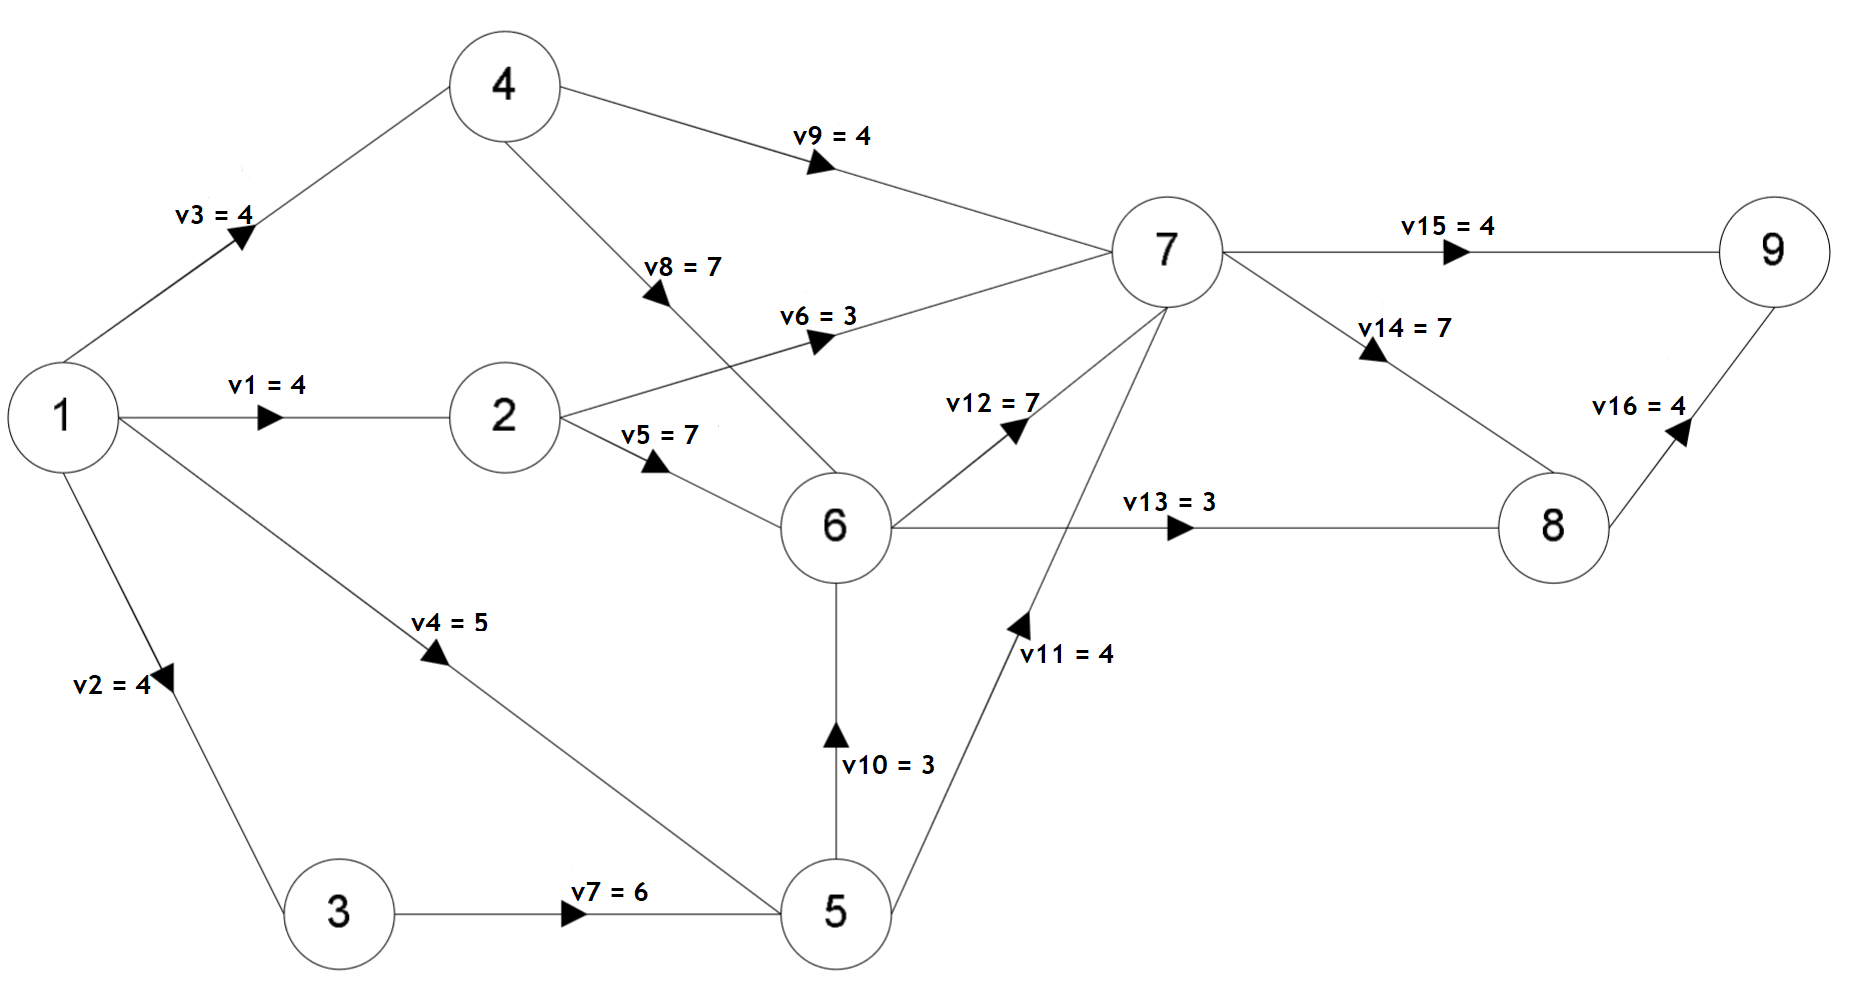
\includegraphics[scale=0.45]{graph-src}
	\caption{Ориентированный граф}
	\label{pic:graph-src}
\end{center}
\end{figure}

\begin{enumerate}
	\item Упорядочить вершины графа – провести разбиение множества вершин графа на непересекающиеся подмножества (уровни), показать уровни на графе.
	
	\item Определить наименьший путь (пути) на графе методом динамического программирования, выделить его на графе.
	
	\item Определить наибольший путь (пути) на графе методом динамического программирования, выделить его на графе.
	
\end{enumerate}

\section{Решение}

\subsection{Разбиение на уровни}

Выполним разбиение множества вершин на уровни:

\begin{equation*}
	A_1 = \{1\},\ \ \ \ \ A_2 = \{2,\ 3,\ 4\},\ \ \ \ A_3 = \{5\}
\end{equation*}

\begin{equation*}
	A_4 = \{6\},\ A_5 = \{7\},\ A_6 = \{8\},\ A_7 = \{9\}
\end{equation*}

Покажем разбиение на графе:

\begin{figure}[H]
\begin{center}
	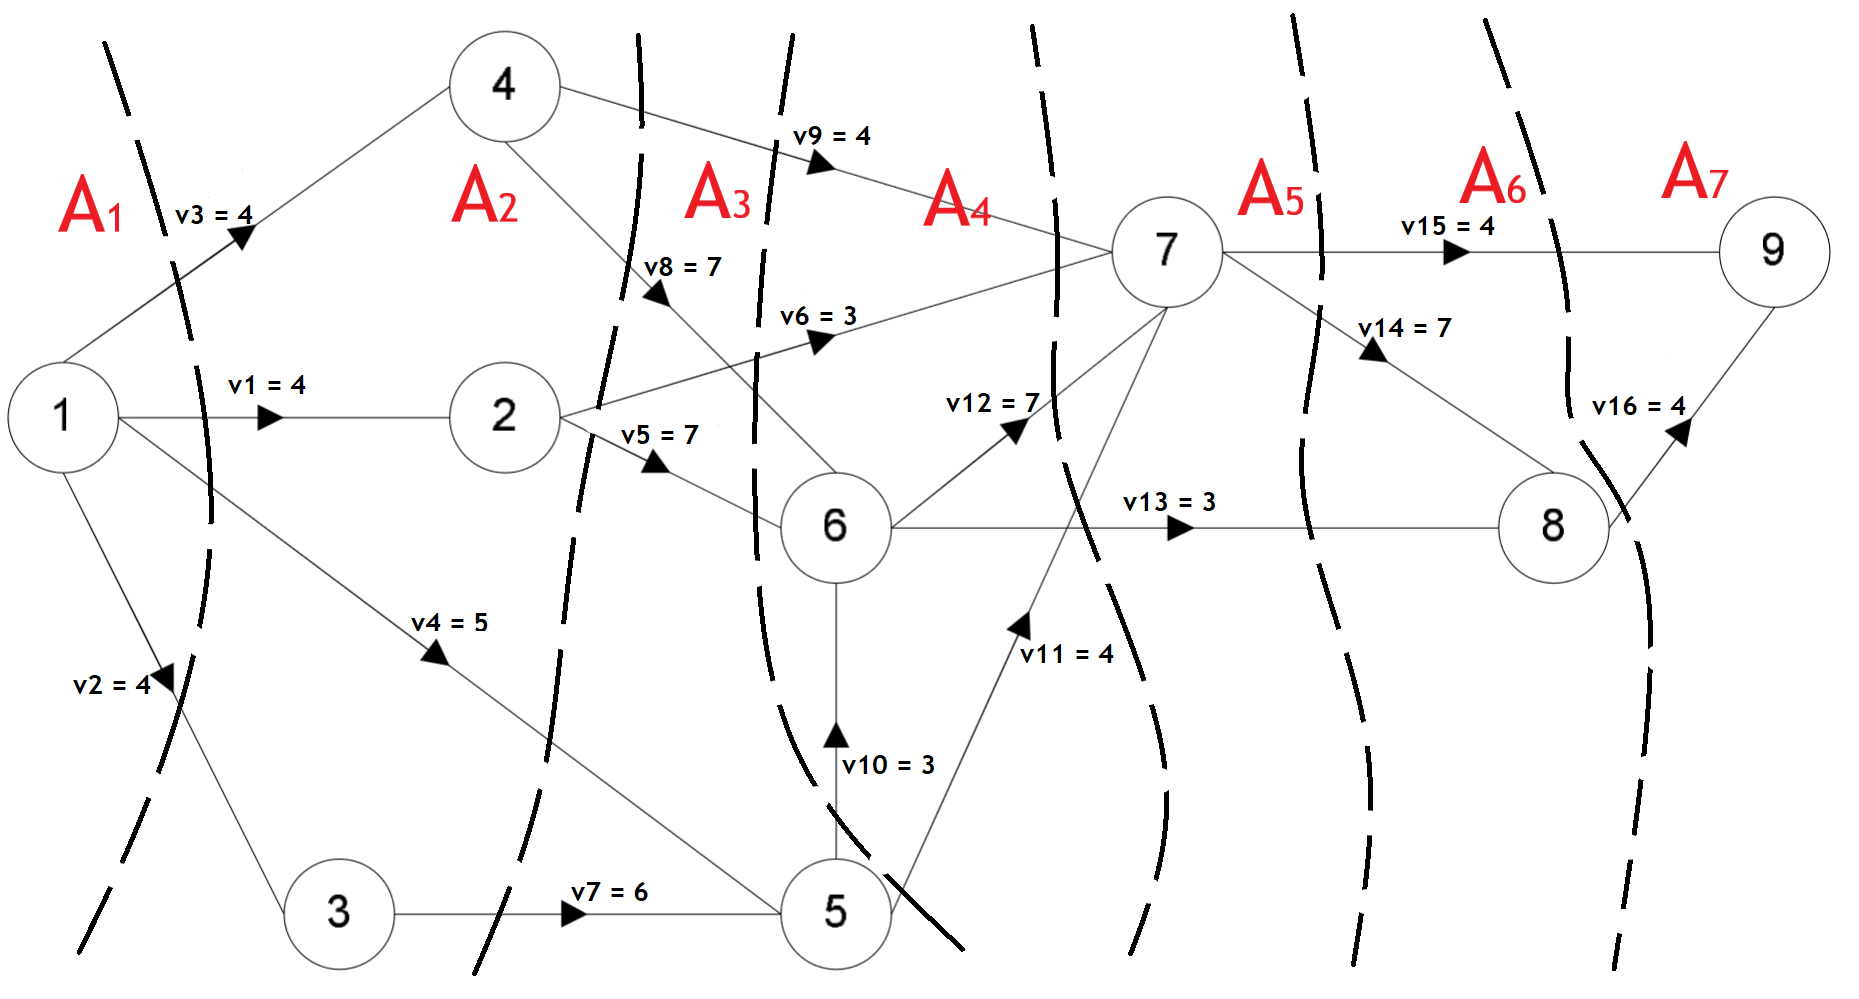
\includegraphics[scale=0.35]{graph-classified}
	\caption{Разбиение на уровни на графе}
	\label{pic:graph-classified}
\end{center}
\end{figure}

\subsection{Наименьший путь}

\begin{equation*}
	l_{VII}(9,\ 9) = l_9 = 0
\end{equation*}

\begin{equation*}
	l_{VI}(8,\ 9) = l_8 = 4 + l_9 = 4 + 0 = 4
\end{equation*}

\begin{equation*}
	l_{V}(7,\ 9) = l_7 = min \begin{pmatrix} 7 + l_8 \\ \underline{4 + l_9} \end{pmatrix} = min \begin{pmatrix} 7 + 4 \\ \underline{4 + 0} \end{pmatrix} = 4
\end{equation*}

\begin{equation*}
	l_{IV}(6,\ 9) = l_6 = min \begin{pmatrix} 7 + l_7 \\ \underline{3 + l_8} \end{pmatrix} = min \begin{pmatrix} 7 + 4 \\ \underline{3 + 4} \end{pmatrix} = 7
\end{equation*}

\begin{equation*}
	l_{III}(5,\ 9) = l_5 = min \begin{pmatrix} 3 + l_6 \\ \underline{4 + l_7} \end{pmatrix} = min \begin{pmatrix} 3 + 7 \\ \underline{4 + 4} \end{pmatrix} = 8
\end{equation*}

\begin{equation*}
	l_{II}(4,\ 9) = l_4 = min \begin{pmatrix} 7 + l_6 \\ \underline{4 + l_7} \end{pmatrix} = min \begin{pmatrix} 7 + 7 \\ \underline{4 + 4} \end{pmatrix} = 8
\end{equation*}

\begin{equation*}
	l_{II}(3,\ 9) = l_3 = 6 + l_5 = 6 + 8 = 14
\end{equation*}

\begin{equation*}
	l_{II}(2,\ 9) = l_2 = min \begin{pmatrix} 7 + l_6 \\ \underline{3 + l_7} \end{pmatrix} = min \begin{pmatrix} 7 + 7 \\ \underline{3 + 4} \end{pmatrix} = 7
\end{equation*}

\begin{equation*}
	l_{I}(1,\ 9) = l_1 = min \begin{pmatrix} \underline{4 + l_2} \\ 4 + l_3 \\ 4 + l_4 \end{pmatrix} = min \begin{pmatrix} \underline{4 + 7} \\ 4 + 14 \\ 4 + 8 \end{pmatrix} = 11
\end{equation*}

Маршрут наименьшего пути: $1 \rightarrow 2 \rightarrow 7 \rightarrow 9$.\\ Отметим его на графе (рис. \ref{pic:min}).

\begin{figure}[H]
\begin{center}
	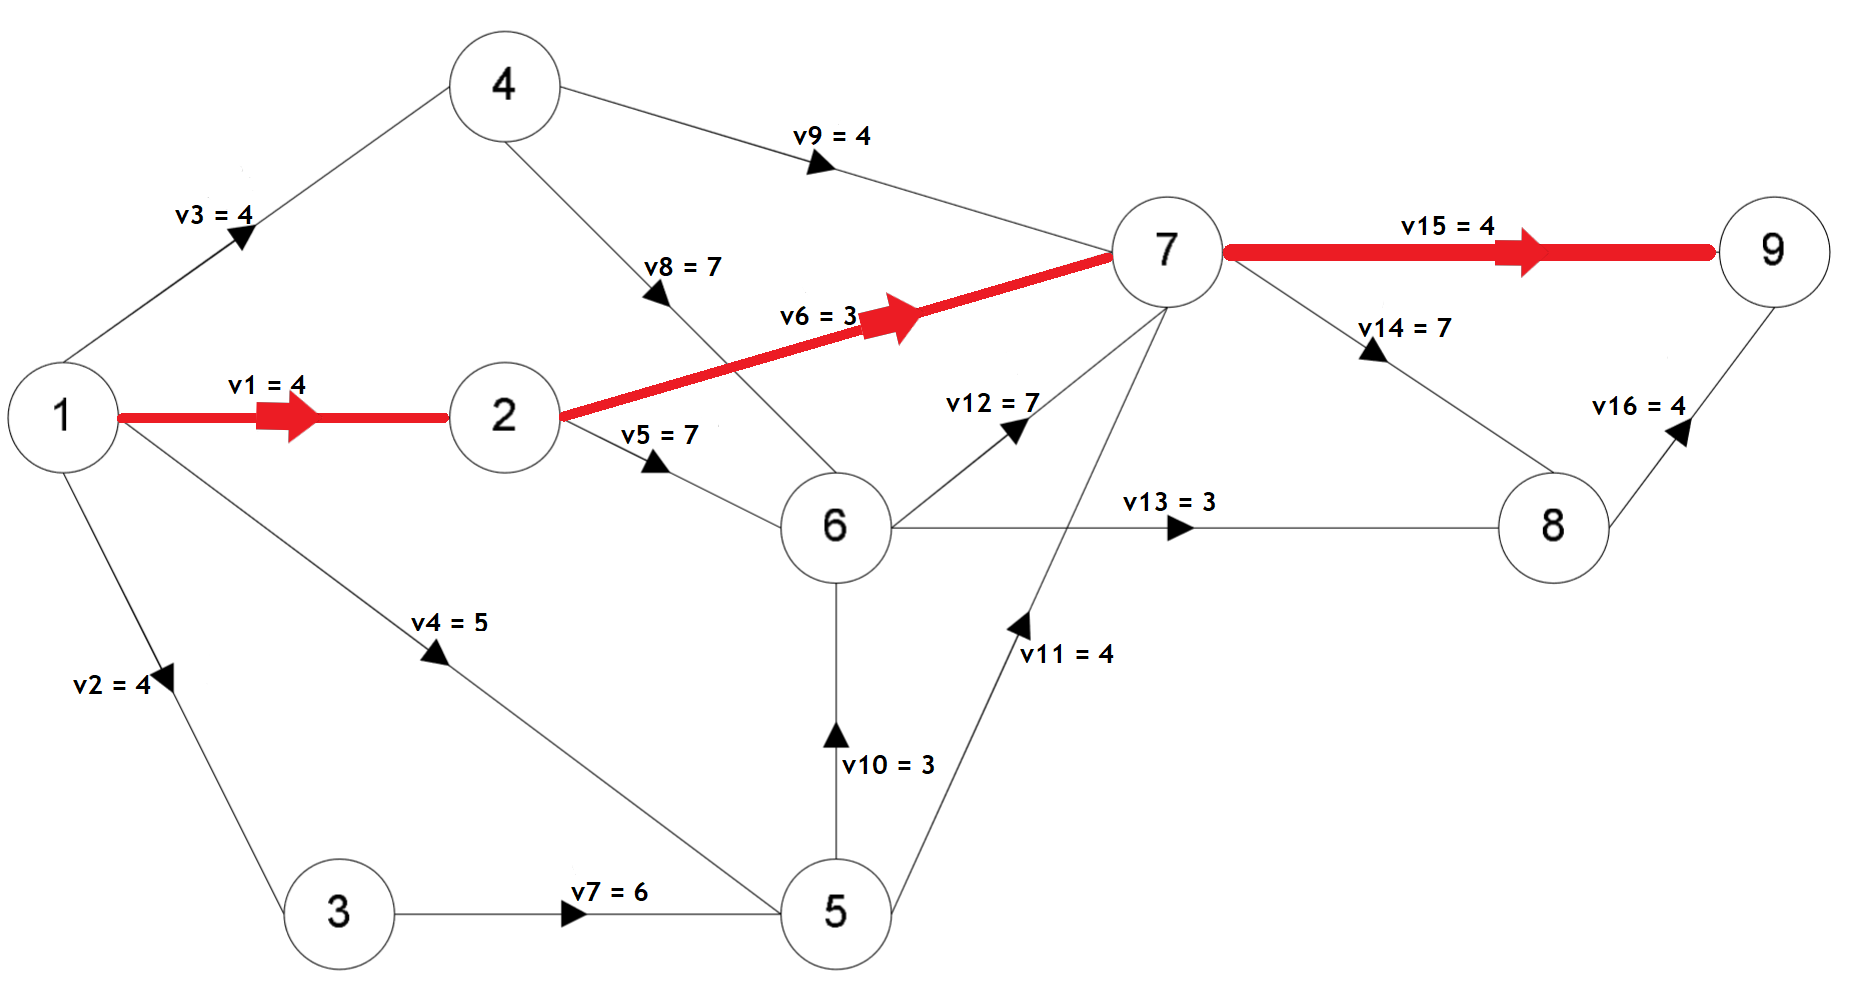
\includegraphics[scale=0.35]{min}
	\caption{Наименьший путь на графе}
	\label{pic:min}
\end{center}
\end{figure}

\subsection{Наибольший путь}

\begin{equation*}
	l_{VII}(9,\ 9) = l_9 = 0
\end{equation*}

\begin{equation*}
	l_{VI}(8,\ 9) = l_8 = 4 + l_9 = 4 + 0 = 4
\end{equation*}

\begin{equation*}
	l_{V}(7,\ 9) = l_7 = max \begin{pmatrix} \underline{7 + l_8} \\ 4 + l_9 \end{pmatrix} = max \begin{pmatrix} \underline{7 + 4} \\ 4 + 0 \end{pmatrix} = 11
\end{equation*}

\begin{equation*}
	l_{IV}(6,\ 9) = l_6 = max \begin{pmatrix} \underline{7 + l_7} \\ 3 + l_8 \end{pmatrix} = max \begin{pmatrix} \underline{7 + 11} \\ 3 + 4 \end{pmatrix} = 18
\end{equation*}

\begin{equation*}
	l_{III}(5,\ 9) = l_5 = max \begin{pmatrix} \underline{3 + l_6} \\ 4 + l_7 \end{pmatrix} = max \begin{pmatrix} \underline{3 + 18} \\ 4 + 11 \end{pmatrix} = 21
\end{equation*}

\begin{equation*}
	l_{II}(4,\ 9) = l_4 = max \begin{pmatrix} \underline{7 + l_6} \\ 4 + l_7 \end{pmatrix} = max \begin{pmatrix} \underline{7 + 18} \\ 4 + 11 \end{pmatrix} = 25
\end{equation*}

\begin{equation*}
	l_{II}(3,\ 9) = l_3 = 6 + l_5 = 6 + 21 = 27
\end{equation*}

\begin{equation*}
	l_{II}(2,\ 9) = l_2 = max \begin{pmatrix} \underline{7 + l_6} \\ 3 + l_7 \end{pmatrix} = max \begin{pmatrix} \underline{7 + 18} \\ 3 + 11 \end{pmatrix} = 25
\end{equation*}

\begin{equation*}
	l_{I}(1,\ 9) = l_1 = max \begin{pmatrix} 4 + l_2 \\ \underline{4 + l_3} \\ 4 + l_4 \end{pmatrix} = max \begin{pmatrix} 4 + 25 \\ \underline{4 + 27} \\ 4 + 25 \end{pmatrix} = 31
\end{equation*}

Маршрут наибольшего пути: $1 \rightarrow 3 \rightarrow 5 \rightarrow 6 \rightarrow 7 \rightarrow 8 \rightarrow 9$.\\ Отметим его на графе (рис. \ref{pic:max}).

\begin{figure}[H]
\begin{center}
	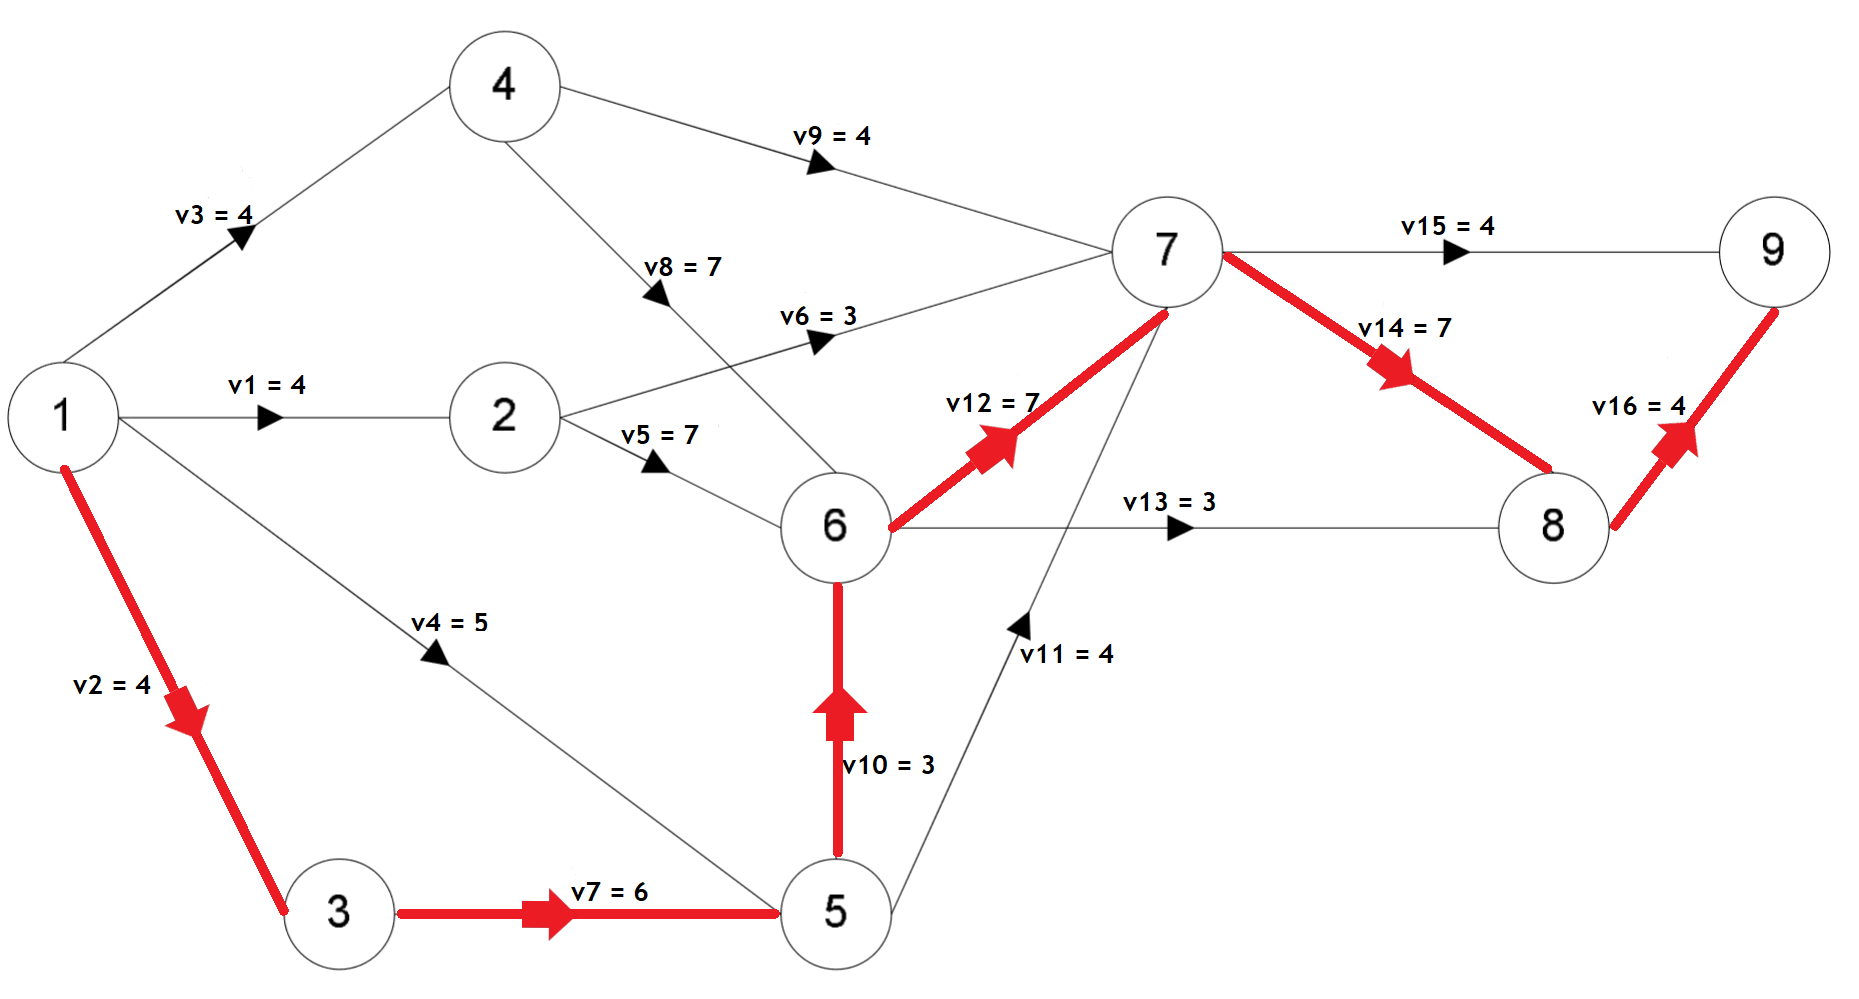
\includegraphics[scale=0.35]{max}
	\caption{Наибольший путь на графе}
	\label{pic:max}
\end{center}
\end{figure}

\end{document}